










\section{Experiment 2}

The aim of this experiment is to see what the cost of SA in a local environment is and if it is additive by the number of suffixes using a self-paced reading study. A local environment means that the target conjunct and the source conjunct for the suspended affix(es) are in the adjacent periphery of the conjoiner. Target conjunct is where the affix is interpreted but phonologically covert and the source conjunct is where it is overt. In the case of Turkish, the source conjunct is the rightmost conjunct as illustrated in (\ref{templateforsuspension}).

\begin{exe}
\ex \label{templateforsuspension}
CONJ1$_{target}$ (conjoiner) CONJ2$_{source}$ 
\end{exe}

SA in the nominal domain is ambiguous except than the SA of {\Case}. SA in the verbal domain, on the other hand, does not result in ambiguity, and the SA capable suffixes can be stacked. This enables me to test the effects, if any, of suspending different number of suffixes. In addition to changing the amount of suffixes, I investigate if the acceptability decreasing effect of the conjoiner \textit{veya} `or' in the first experiment will be reflected by increases in reading times.

There is one concern with using verbal domain for SA. The target conjunct can only be reduced to a verb plus a participle morpheme. These participle morphemes can have {\Tsg} agreement interpretations on their own. Should an effect arise in SA amount changes, it might be related to the mismatches between the first and second conjuncts instead of SA. There are additional conditions to meet this concern. These conditions are formed by changing an aspect or agreement of the first conjunct. This provides a contrast in terms of distinguishing an effect of suspension from feature mismatches. I lay out the experiment and analysis of the results in the following subsections.


\subsection{Participants}

The participants were 160 students from Boğaziçi University who are native speakers of Turkish. In exchange for their participation they received 1 point to their overall course score with the consent of the course's instructor.


\subsection{Materials}

The experiment comprised of three variables. The first variable was the Amount of SA with the levels: No SA, One SA, and Full SA.
In No SA, no suffix is suspended. In One SA, only one suffix is suspended. In Full SA, two suffixes are suspended. The second variable is the Conjoiner with the levels: \textit{ve} `and' and \textit{veya} `or'. The third variable is Contrast with the levels: Contrast and Parallel (No\_SA). In this last variable one of the suffixes in the first conjunct is altered to have a grammatical feature mismatch between the conjuncts. This contrast is only performed on the No SA conditions. This resulted in an experiment design with 4x2 conditions combining the amount of SA and conjoiner type, plus two conditions where there is a contrasting first conjunct for No SA condition. There were 24 distinct items together with 48 filler items. All experimental and filler items were grammatical. A latin square design by condition was applied, forming 8 lists of 24. This resulted in each participant seeing only 24 experimental items and 48 fillers. All the experimental items had a four-word pre and four-word post conjunction regions. (\ref{selfpacedtemplate}) shows a template for an experimental item. In (\ref{selfpacedexamples}), I give an example set of experimental items with all the conditions. All the experimental items and fillers had a comprehension question with half of them having "yes" and the other half having "no" as the correct answer. I carried out the experiment using ibexfarm \citep{drummond2013ibex}. For the full list of items and fillers (1-24 and 100-148) see Appendix \ref{selfpaceditems}.

\begin{exe}
\ex \label{selfpacedtemplate}
4WORDS CONJ1-$\alpha$-$\beta$ \textit{ve/veya} CONJ2-$\alpha$-$\beta$ 4WORDS

\ex \label{selfpacedexamples}
    \begin{xlist}
  \ex No SA:{\And}/{\Or}\\* 
  \gll \ldots yap-sa-ymış-ım ve/veya gönder-se-ymiş-im \ldots \\ 
  \ldots do-{\Cond}-{\Prf}-{\Fsg} {\And}/{\Or} send-{\Cond}-{\Prf}-{\Fsg} \ldots \\
  \glt ${}$

  \ex One SA:{\And}/{\Or}\\*
  \gll \ldots yap-sa-ymış ve/veya gönder-se-ymiş-im \ldots \\ 
  \ldots do-{\Cond}-{\Prf} {\And}/{\Or} send-{\Cond}-{\Prf}-{\Fsg} \ldots \\
  \glt ${}$
  
  \ex Full SA:{\And}/{\Or}\\*
  \gll \ldots yap-sa ve/veya gönder-se-ymiş-im \ldots \\ 
  \ldots do-{\Cond} {\And}/{\Or} send-{\Cond}-{\Prf}-{\Fsg} \ldots \\
  \glt ${}$
  
  \ex Contrast:{\And}/{\Or}\\*
  \gll \ldots yap-sa-ymış-ız ve/veya gönder-se-ymiş-im \ldots \\ 
  \ldots do-{\Cond}-{\Prf}-{\Fpl} {\And}/{\Or} send-{\Cond}-{\Prf}-{\Fsg} \ldots \\
    \end{xlist}
\end{exe}


\subsection{Procedure}

Participants were provided with a link to the experiment prompting them with a consent page. Upon giving consent participants went through 5 practice items and then they were prompted again for the beginning of the experiment. Each trial proceeded by the participants pushing the "space" key, for each key stroke a word at the center of the screen appeared and by each key stroke it was replaced with the following word in the sentence. After the sentence was read, the participants were presented with a statement that was either true or false according to the sentence they read. The statement was made about a dependency that was formed within the sentence. This could have been a modification of a noun or the verb, or the argument relations within the sentence. Participants professed their decision by pushing "Q" key for "yes" and "P" key for "no" on the keyboard. The experiment only recorded word reading times, responses, and response times. After the experiment was done, the participants were redirected to a separate page where they provided their student information to be relayed to the course's professor for the extra credit. This is kept separate of the experiment results, keeping participant information and experimental data anonymous.

\subsection{Results}

The results were recorded onto a csv file and imported to R \citep{team2013r} for data cleaning, aggregation, and analysis. Two items with a typo are excluded from the data (they do not count in initial data points). The data consisted of 38720 points before cleaning. . 4 participants whose accuracies were below 70\% are excluded from the data. After these exclusions, 15.48\% of the trials which had incorrect answers for the comprehension question are excluded from data analysis. The trials in which a word had a reading time that was outside 100-3000 milliseconds were considered outliers and those trials are also excluded. The whole cleaning resulted in the loss of 25.03\% of the data. In Figure \ref{fig:secondplot}, I give the average reading times per word with a representative sentence for the conditions of suspension amount.

\begin{knitrout}
\definecolor{shadecolor}{rgb}{0.969, 0.969, 0.969}\color{fgcolor}\begin{figure}[hbt!]

{\centering 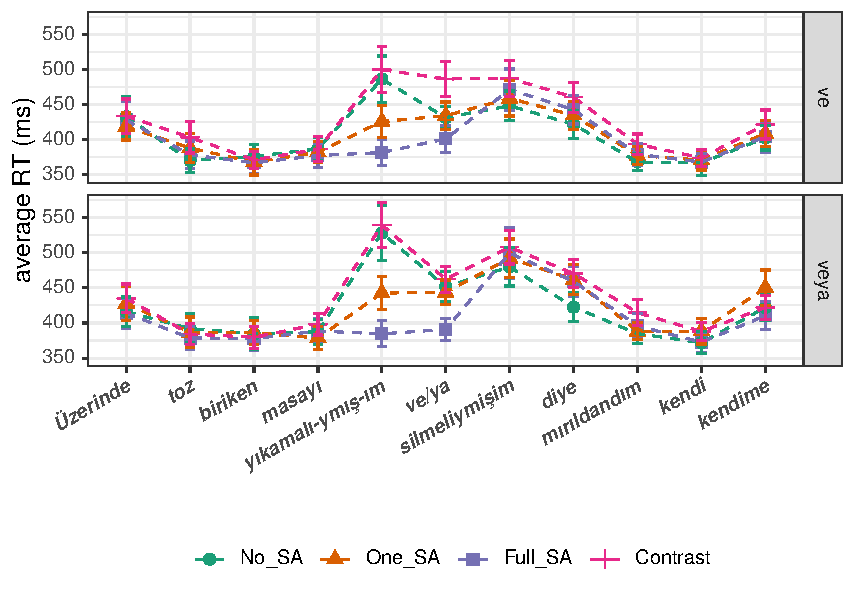
\includegraphics[]{experiments/selfpaced/report/figure/secondplot-1.pdf} 

}

\caption[Average reading times of a sentence for all categories(No SA|One SA|Full SA|Contrast) and conjoiners(ve|veya)]{Average reading times of a sentence for all categories(No SA|One SA|Full SA|Contrast) and conjoiners(ve|veya)}\label{fig:secondplot}
\end{figure}


\end{knitrout}

The critical region in all the sentences is the 7$^{th}$ word. In the case of Figure \ref{fig:secondplot} it is \textit{silmeliymişim} `(I) should have cleaned (something)'. The spillover region is the two words after the critical region. In this case the words \textit{diye} `saying that' and \textit{mırıldandım} ` (I) mumbled'. In Figure \ref{fig:thirdplot}, I give the average reading times of the critical and spillover region words by experimental conditions.

\begin{knitrout}
\definecolor{shadecolor}{rgb}{0.969, 0.969, 0.969}\color{fgcolor}\begin{figure}[hbt!]

{\centering 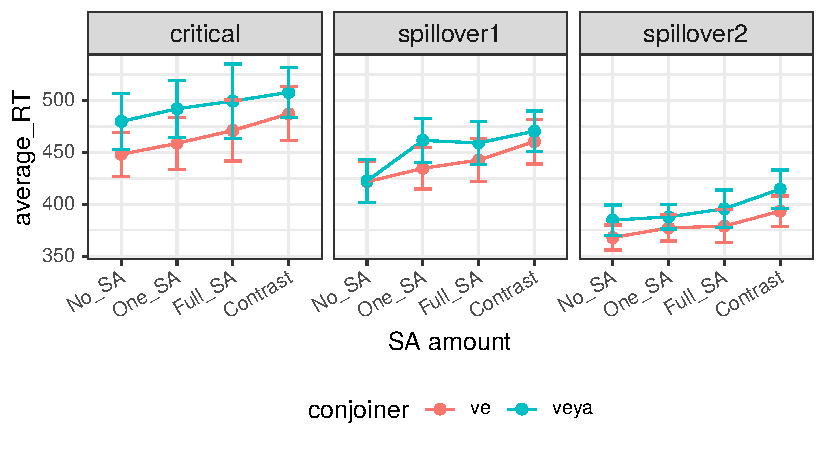
\includegraphics[]{experiments/selfpaced/report/figure/thirdplot-1.pdf} 

}

\caption[Average reading times of critical and spillover regions for all categories(No SA|One SA|Full SA|Contrast) and conjoiners(ve|veya)]{Average reading times of critical and spillover regions for all categories(No SA|One SA|Full SA|Contrast) and conjoiners(ve|veya)}\label{fig:thirdplot}
\end{figure}


\end{knitrout}

There is an increase in critical and spillover regions with the conjoiner \textit{veya} `or'. The amount of suspension does not display a similar trend in all the regions. In the critical region and the first spillover word, there is a slight increase by the number suspended suffixes. Contrasting sentences have higher reading times compared to suspension of one and two suffixes. This indicates that feature mismatches between the conjuncts lead to different processes other than SA.


For more inference on the effects of SA, I fit 3 linear mixed models for the reading times of the critical and spillover region words. I used SA amount and Conjoiner as predictors with random effects for subject and item. I used sliding differences contrasts for the SA amount, and sum contrast for the Conjoiner. Sliding differences mean that the comparisons are made between the levels of the differences. This follows from the expectation of varying effects depending on the SA amount, which is an incremental but not a categorical change. I give the models' results for SA amount in Figure \ref{fig:targetmodels}. The model results indicate an increase in spillover region for the suspension of one suffix, with no additive effects by suspending one more suffix. The conjoiner \textit{veya} `or' increased reading times consistently in all regions.

\begin{knitrout}
\definecolor{shadecolor}{rgb}{0.969, 0.969, 0.969}\color{fgcolor}\begin{figure}[hbt!]

{\centering 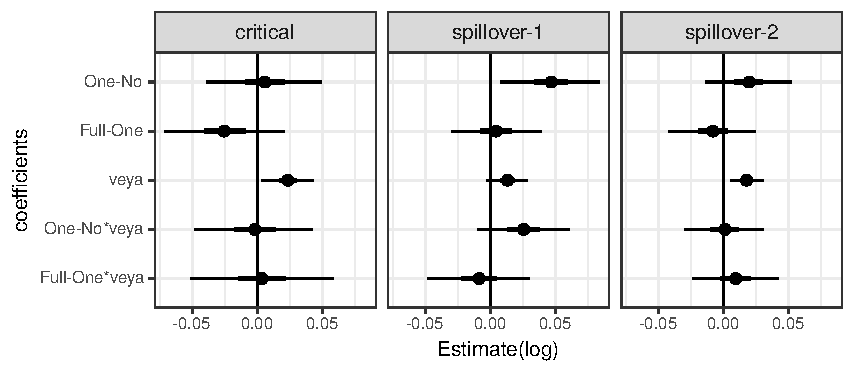
\includegraphics[]{experiments/selfpaced/report/figure/targetmodels-1.pdf} 

}

\caption[Second experiment, model results for the SA amount conditions fit to reading times with the predictors SA amount(No SA|One SA|Full SA) and Conjoiner(ve|veya)]{Second experiment, model results for the SA amount conditions fit to reading times with the predictors SA amount(No SA|One SA|Full SA) and Conjoiner(ve|veya)}\label{fig:targetmodels}
\end{figure}


\end{knitrout}


In addition to the effects of SA, I fit another 3 models for the reading times of the critical and spillover region words using feature match between conjuncts and conjoiner as predictors with random affects for subject and item. I used sliding difference for feature match, comparing Contrast to No\_SA, and sum contrast for the conjoiner. The results indicate an increase in reading times in Contrast conditions in all regions, with an increase in reading times by the conjoiner \textit{veya} `or' only in the critical region and the second spillover region word.

\begin{knitrout}
\definecolor{shadecolor}{rgb}{0.969, 0.969, 0.969}\color{fgcolor}\begin{figure}[hbt!]

{\centering 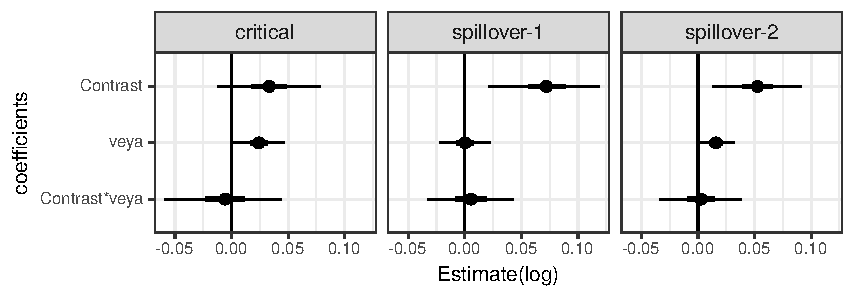
\includegraphics[]{experiments/selfpaced/report/figure/contrastmodels-1.pdf} 

}

\caption[Second experiment, model results for the feature mismatching conjuncts fit to reading times with the predictors Contrast(Contrast|No SA) and Conjoiner(ve|veya)]{Second experiment, model results for the feature mismatching conjuncts fit to reading times with the predictors Contrast(Contrast|No SA) and Conjoiner(ve|veya)}\label{fig:contrastmodels}
\end{figure}


\end{knitrout}

Figures \ref{fig:targetmodels} and \ref{fig:contrastmodels} indicate that suspending an affix and feature mismatches between conjuncts increase reading times. I fit 3 other models to compare only One SA and Contrast conditions in all the regions with random effects for subject and item. This time I used sum contrasts across the board. If the two levels behave the same, the comparison should result in indifference between One SA and Contrast. I give the models' results in Figure \ref{fig:saVcontrast}. The results indicate increased reading times in Contrast conditions compared to One SA. This differentiates the operation of SA and feature mismatches between the conjuncts. 

\begin{knitrout}
\definecolor{shadecolor}{rgb}{0.969, 0.969, 0.969}\color{fgcolor}\begin{figure}[hbt!]

{\centering 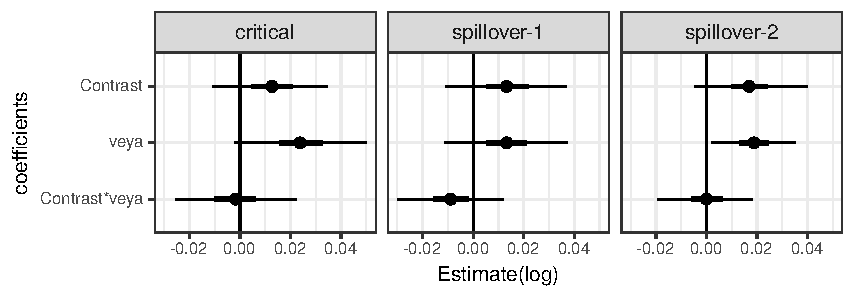
\includegraphics[]{experiments/selfpaced/report/figure/saVcontrast-1.pdf} 

}

\caption[Second experiment, model results for the comparison of suspending an affix and feature mismatching conjuncts fit to reading times with the predictors of Category(Contrast|One SA) and Conjoiner(ve|veya)]{Second experiment, model results for the comparison of suspending an affix and feature mismatching conjuncts fit to reading times with the predictors of Category(Contrast|One SA) and Conjoiner(ve|veya)}\label{fig:saVcontrast}
\end{figure}


\end{knitrout}

\subsection{Analysis}

In this experiment, the main aim was to identify the cost of SA. The results indicate that suspending a suffix is costly but it is not additive. The conjoiner \textit{veya} `or' increased reading times, this is a similar trend of decreasing acceptabilities in the first experiment. The feature mismatches between the conjuncts also lead to increased processing cost but they are greater than those of suspension. In the first experiment this effect is directly realted to SA, because the response was directly related to SA. In this experiment the main effect of the conjoiner in reading times can not be tied to SA. An increase in reading times can be caused by the semantic difference between the two conjoiners \textit{ve} `and' and \textit{veya} `or'. This means that the conjoiner effect in this experiment is not related to SA directly. If there was such a relation, the conjoiner \textit{veya} `or' and the suspension conditions should have had an interaction effect, presumably an increase in reading times for suspending suffixes in an environment formed by the conjoiner \textit{veya} `or'.









